% Paquets généraux
\documentclass[a4paper,12pt,titlepage]{article}
\usepackage[T1]{fontenc}
\usepackage[utf8]{inputenc}
\usepackage[french]{babel}
\usepackage[gen]{eurosym}
%\usepackage[dvips]{graphicx}
\usepackage{fancyhdr}
\usepackage{pdfpages} 
\usepackage{multido}
\usepackage{hyperref}
%\usepackage{textcomp}
%\usepackage{aeguill}
\usepackage{schemabloc}
\usepackage[bitstream-charter]{mathdesign}

\newcommand{\id}{54}
\newcommand{\nom}{Liaisons mécaniques}
\newcommand{\sequence}{04}
\newcommand{\num}{01}
\newcommand{\type}{TP}
\newcommand{\descrip}{Modélisation d'un solide. Comportement des liaisons mécaniques. Modéliser les mécanismes du laboratoire par un schéma cinématique, paramétré.}
\newcommand{\competences}{A3-C4: Analyse d'architecture et de comportement \\ &  Mod1-C1: Isolement d'un solide ou d'un système de solides \\ &  Mod2-C10-1: Modèle de solide indéformable \\ &  Mod2-C11: Modélisation géométrique et cinématique des mouvements entre solides indéformables \\ &  Mod2-C12: Modélisation cinématique des liaisons entre solides \\ &  Mod2-C15: Modélisation des actions mécaniques \\ &  Rés-C6: Utilisation d'un solveur ou d'un logiciel multi physique \\ &  Com1-C1: Différents descripteurs introduits dans le programme \\ &  Com2-C4: Outils de communication}
\newcommand{\nbcomp}{9}
\newcommand{\systemes}{Plateforme Stewart}
\newcommand{\systemessansaccent}{Plateforme Stewart}
\newcommand{\ilot}{2}
\newcommand{\ilotstr}{02}
\newcommand{\dossierilot}{\detokenize{Ilot_02 Plateforme Stewart}}
\newcommand{\imageun}{Plateforme}

\newcommand{\urlsysteme}{\href{https://www.costadoat.fr/systeme/57}{Ressources système}}
\newcommand{\matlabsimscape}{\href{https://github.com/Costadoat/Sciences-Ingenieur/raw/master/Systemes/Plateforme Stewart/Plateforme_Stewart_Simscape.zip}{Modèle Simscape}}
\newcommand{\solidworks}{\href{https://github.com/Costadoat/Sciences-Ingenieur/raw/master/Systemes/Plateforme Stewart/Plateforme_Stewart_Solidworks.zip}{Modèle Solidworks}}
\newcommand{\edrawings}{\href{https://github.com/Costadoat/Sciences-Ingenieur/raw/master/Systemes/Plateforme Stewart/Plateforme_Stewart.EASM}{Modèle eDrawings}}
\newcommand{\test}{Stewart_param1}
\newcommand{\testi}{Stewart_param2}
\newcommand{\testii}{Stewart_param3}
\newcommand{\testiii}{Stewart_param4}
\newcommand{\testiiii}{Stewart_euler}

\newcommand{\auteurun}{Renaud Costadoat}
\newcommand{\auteurdeux}{Françoise Puig}
\newcommand{\institute}{Lycée Dorian}


\usepackage{color}
\usepackage{xcolor}
\usepackage{colortbl}
\usepackage{helvet}
\renewcommand{\familydefault}{\sfdefault}
\usepackage{amsfonts}
\usepackage{amsmath}
%\usepackage{xspace}
\usepackage{varioref}
\usepackage{tabularx}
%\usepackage{floatflt}
\usepackage{graphics}
\usepackage{wrapfig}
\usepackage{textcomp}
\usepackage{tikz}
\usepackage{wrapfig}
\usepackage{gensymb}
\usepackage[european]{circuitikz}
\usetikzlibrary{babel}
\usepackage{ifthen}
\usepackage{cancel}
\usepackage{etoolbox}
\usepackage{multirow}
%\usepackage{boxedminipage}
\definecolor{gris25}{gray}{0.75}
\definecolor{bleu}{RGB}{18,33,98}
\definecolor{bleuf}{RGB}{42,94,171}
\definecolor{bleuc}{RGB}{231,239,247}
\definecolor{rougef}{RGB}{185,18,27}
\definecolor{rougec}{RGB}{255,188,204}%255,230,231
\definecolor{vertf}{RGB}{103,126,82}
\definecolor{vertc}{RGB}{220,255,191}
\definecolor{forestgreen}{rgb}{0.13,0.54,0.13}
\definecolor{blcr}{rgb}{0.59,0.69,0.84}
\definecolor{blfr}{rgb}{0.32,0.51,0.75}
\definecolor{orfr}{rgb}{0.90,0.42,0.15}
\definecolor{orcr}{rgb}{0.90,0.65,0.50}
\definecolor{orangef}{rgb}{0.659,0.269,0.072}
\definecolor{orange}{rgb}{0.58,0.35,0.063}
\definecolor{orangec}{rgb}{0.43,0.32,0.25}
\definecolor{rcorrect}{rgb}{0.6,0,0}
\definecolor{sequence}{rgb}{0.75,0.75,0.75}
\definecolor{competences}{rgb}{0.61,0.73,0.35}
\definecolor{grisf}{HTML}{222222}
\definecolor{grisc}{HTML}{636363}
\definecolor{normal}{HTML}{4087c4}
\definecolor{info}{HTML}{5bc0de}
\definecolor{success}{RGB}{92,184,92}
\definecolor{warning}{RGB}{240,173,78}
\definecolor{danger}{RGB}{217,83,79}
\hypersetup{                    % parametrage des hyperliens
    colorlinks=true,                % colorise les liens
    breaklinks=true,                % permet les retours à la ligne pour les liens trop longs
    urlcolor= blfr,                 % couleur des hyperliens
    linkcolor= orange,                % couleur des liens internes aux documents (index, figures, tableaux, equations,...)
    citecolor= forestgreen                % couleur des liens vers les references bibliographiques
    }

% Mise en page
\pagestyle{fancy}

\setlength{\hoffset}{-18pt}

\setlength{\oddsidemargin}{0pt} 	% Marge gauche sur pages impaires
\setlength{\evensidemargin}{0pt} 	% Marge gauche sur pages paires
\setlength{\marginparwidth}{00pt} 	% Largeur de note dans la marge
\setlength{\headwidth}{481pt} 	 	% Largeur de la zone de tête (17cm)
\setlength{\textwidth}{481pt} 	 	% Largeur de la zone de texte (17cm)
\setlength{\voffset}{-18pt} 		% Bon pour DOS
\setlength{\marginparsep}{7pt}	 	% Séparation de la marge
\setlength{\topmargin}{-30pt} 		% Pas de marge en haut
\setlength{\headheight}{35pt} 		% Haut de page
\setlength{\headsep}{20pt} 		% Entre le haut de page et le texte
\setlength{\footskip}{30pt} 		% Bas de page + séparation
\setlength{\textheight}{700pt} 		% Hauteur de l'icone zone de texte (25cm)
\setlength\fboxrule{1 pt}
\renewcommand{\baselinestretch}{1}
\setcounter{tocdepth}{1}
\newcommand{\cadre}[2]
{\fbox{
  \begin{minipage}{#1\linewidth}
   \begin{center}
    #2\\
   \end{center}
  \end{minipage}
 }
}

\newcounter{num_quest} \setcounter{num_quest}{0}
\newcounter{num_rep} \setcounter{num_rep}{0}
\newcounter{num_cor} \setcounter{num_cor}{0}

\newcommand{\question}[1]{\refstepcounter{num_quest}\par
~\ \\ \parbox[t][][t]{0.15\linewidth}{\textbf{Question \arabic{num_quest}}}\parbox[t][][t]{0.93\linewidth}{#1}\par
}


\newcommand{\reponse}[1]
{\refstepcounter{num_rep}
\noindent
\rule{\linewidth}{.5pt}
\textbf{Question \arabic{num_rep}:}
\multido{\i=1+1}{#1}{~\ \\}
}

\newcommand{\cor}
{\refstepcounter{num_cor}
\noindent
\rule{\linewidth}{.5pt}
\textbf{Question \arabic{num_cor}:} \\
}

\newcommand{\titre}[1]
{\begin{center}
\cadre{0.8}{\huge #1} 
\end{center}
}


% En tête et pied de page
\fancypagestyle{normal}{%
  \fancyhf{}
\lhead{\nom}
\rhead{
\includegraphics[width=2cm]{../../img/logo}\hspace{2pt}}
\ifdef{\auteurdeux}{\lfoot{\auteurun,\auteurdeux}}{\lfoot{\auteurun}}
\cfoot{Page \thepage}}

\fancypagestyle{correction}{%
  \fancyhf{}
  \lhead{\colorbox{danger}{\begin{minipage}{0.65\paperwidth} \textcolor{white}{\textbf{Correction}} \end{minipage}} }
  \rhead{
\includegraphics[width=2cm]{../../img/logo}}
  \ifdef{\auteurdeux}{\lfoot{\auteurun,\auteurdeux}}{\lfoot{\auteurun}}
  \rfoot{\colorbox{danger}{\begin{minipage}{0.5\paperwidth} \begin{flushright}\textcolor{white}{\textbf{Correction}}\end{flushright} \end{minipage}} }}

\renewcommand{\footrulewidth}{0.4pt}

\usepackage{eso-pic}
\newcommand{\BackgroundPic}{%
\put(0,0){%
\parbox[b][\paperheight]{\paperwidth}{%
\vfill
\begin{center}
\hspace{0.5cm}\vspace{0.5cm}

\includegraphics[width=\paperwidth,height=\paperheight,%
keepaspectratio]{../../img/fond3}%
\end{center}
\vfill
}}}

\newcommand{\BackgroundPicdeux}{%
\put(25,-30){%
\parbox[b][\paperheight]{\paperwidth}{%
\vfill
\begin{center}

\includegraphics[width=\paperwidth,height=\paperheight,%
keepaspectratio]{../../img/fond4}%
\end{center}
\vfill
}}}

\begin{document}

\pagestyle{empty}

\vspace*{-3\baselineskip}

\AddToShipoutPicture*{\BackgroundPic}

\ifdef{\auteurdeux}{\begin{tabular}{>{\columncolor{gray!00}}m{.3\linewidth} m{.3\linewidth} >{\columncolor{gray!00}}m{.3\linewidth}}
Séquence : \sequence &  \multirow{3}{*}{\hspace{1cm}
\includegraphics[height=1.5cm]{../../img/logo}} &  \begin{flushright} \multirow{4}{*}{\hspace{1cm}
\includegraphics[height=4cm]{img/qrcode}}\end{flushright}\\
Document : \type\num \\
 \institute \\
 \auteurun\\
 \auteurdeux
\end{tabular}}{\begin{tabular}{>{\columncolor{gray!00}}m{.3\linewidth} m{.3\linewidth} >{\columncolor{gray!00}}m{.3\linewidth}}
Séquence : \sequence &  \multirow{3}{*}{\hspace{1cm}
\includegraphics[height=1.5cm]{../../img/logo}} &  \begin{flushright} \multirow{4}{*}{\hspace{1cm}
\includegraphics[height=4cm]{img/qrcode}}\end{flushright}\\
Document : \type\num \\
 \institute \\
 \auteurun
\end{tabular}}

\vspace{1cm}

\ifdef{\prive}{\begin{center}\colorbox{danger}{\Huge{Avec Correction}}\end{center}}{}

\begin{center}\huge{\nom}\end{center}

\vspace{2cm}

\ifdef{\imagedeux}{\begin{minipage}{0.49\linewidth}}{}
\begin{center}\includegraphics[height=5cm]{/home/renaud/Documents/Renaud/GitHub/django_education/systemes/\imageun}\end{center}
\ifdef{\imagedeux}{\end{minipage}\hfill
\begin{minipage}{0.49\linewidth}
\begin{center}\includegraphics[height=5cm]{/home/renaud/Documents/Renaud/GitHub/django_education/systemes/\imagedeux}\end{center}
\end{minipage}}{}

\vspace{5cm}


\begin{tabular}{p{.15\linewidth} >{\columncolor{white}}p{.8\linewidth}}
    \rowcolor{gray!20}
    Référence & S\sequence\ - \type\num \\
    Compétences & \competences \\
 	\rowcolor{gray!20}
    Description & \descrip \\
    Système & \systemes
  \end{tabular}

\newpage

\AddToShipoutPicture{\BackgroundPicdeux}

\pagestyle{normal}

\section{Borne de calage}

\subsection{Création d'une esquisse}

\begin{minipage}{0.6\linewidth}
Croquis de la pièce, appelée "Corps", en perspective avec les cotes principales.
\end{minipage}
\hfill
\begin{minipage}{0.35\linewidth}
\begin{center}
 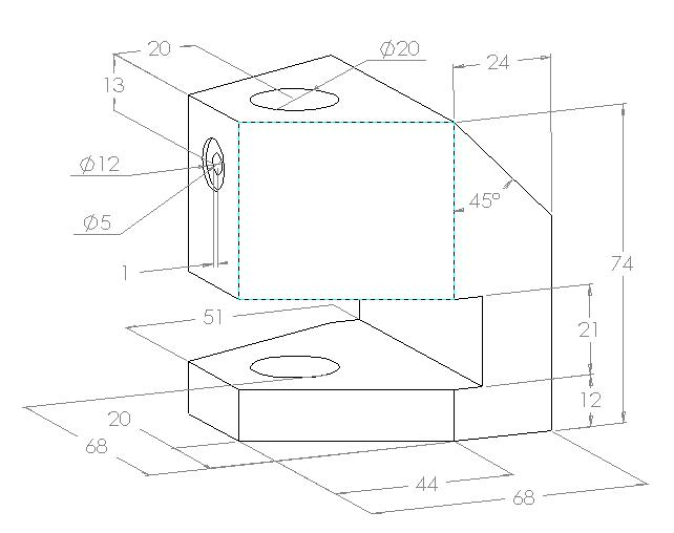
\includegraphics[width=4cm]{img/001_4}
\end{center}
\end{minipage}

\begin{minipage}{0.75\linewidth}
\begin{itemize}
 \item Créez un nouveau fichier pièce
  \begin{itemize}
  \item Enregistrez votre travail sous : "Borne de calage/Corps"
  \end{itemize}
 \item Créer un volume de base
  \begin{itemize}
  \item Ouvrir une esquisse,
  \item Tracer l'esquisse du volume de base,
  \item Réalisez le contour fermé suivant en plaçant le premier point sur l'origine.
  \end{itemize} 
 \item Coter l'esquisse
  \begin{itemize}
  \item Cotez l'esquisse avec l'outil cotation largeur 68 mm, hauteur 74 mm.
  \end{itemize}
\end{itemize}
\end{minipage}
\hfill
\begin{minipage}{0.23\linewidth}
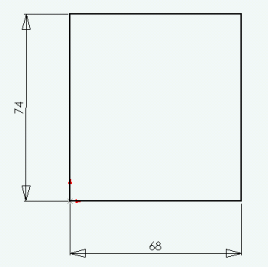
\includegraphics[width=0.9\linewidth]{img/002_5}
\end{minipage}

\subsection{Création d'un volume}

\begin{minipage}{0.75\linewidth}
\begin{itemize}
 \item Créer le bossage extrusion
  \begin{itemize}
  \item Sélectionnez la fonction volumique base/bossage extrudé,
  \item Dans la fenêtre de la fonction volumique base/bossage extrudé,
    \begin{itemize}
    \item Réglez la condition d'extrusion sur plan milieu
    \item Réglez la longueur d'extrusion à la valeur de 68 mm
    \item Validez
    \end{itemize}
  \end{itemize}
 \item Après avoir validez vous pouvez renommer la fonction volumique dont l'ancien nom devient bleu. (s'il n'est pas bleu vous pouvez le sélectionner en double-cliquant lentement sur l'ancien nom)
 \item Nommez la fonction volumique : "Volume de base".
\end{itemize}
\end{minipage}
\hfill
\begin{minipage}{0.23\linewidth}
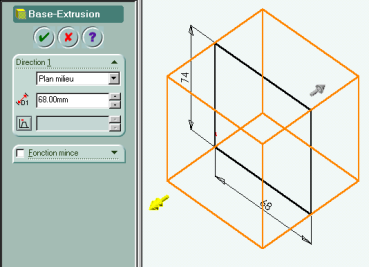
\includegraphics[width=0.9\linewidth]{img/003_3} \\ \vfill
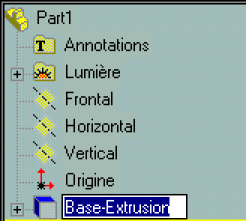
\includegraphics[width=0.9\linewidth]{img/004_3} \\ \vfill
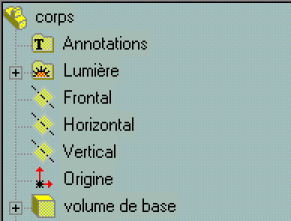
\includegraphics[width=0.9\linewidth]{img/005}
\end{minipage}

\subsection{Création d'une rainure}

\textbf{Esquisse}

~\

\begin{minipage}{0.75\linewidth}
\begin{itemize}
 \item Orienter l'esquisse face à vous, pour cela choisissez l'icône "Normal à",
 \item Choisir l'icône esquisse,
 \item Tracer un rectangle correspondant à la rainure souhaitée à l'aide de l'outil,
 \item Coter l'esquisse avec l'outil cotation largeur 51mm, hauteur 21 mm,
 \item Coter en position la rainure, horizontalement et verticalement.
\end{itemize}
\end{minipage}
\hfill
\begin{minipage}{0.23\linewidth}
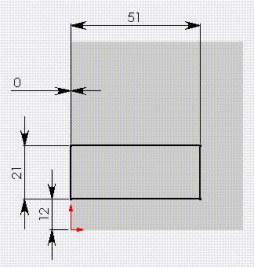
\includegraphics[width=0.9\linewidth]{img/008}
\end{minipage}

\textbf{Volume}

~\

\begin{minipage}{0.75\linewidth}
\begin{itemize}
 \item Sélectionnez la fonction volumique enlèvement matière extrudé
 \item Dans la fenêtre de la fonction :
 \begin{itemize}
 \item Régler la condition d'enlèvement sur A travers tout
 \item Valider
 \end{itemize}
 \item Nommez la fonction volumique : rainure.
\end{itemize}
\end{minipage}
\hfill
\begin{minipage}{0.23\linewidth}
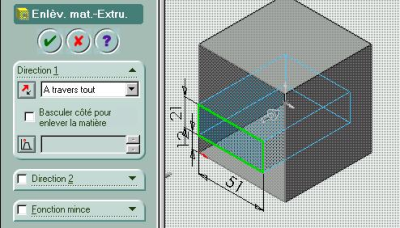
\includegraphics[width=0.9\linewidth]{img/009}
\end{minipage}

\subsection{Création d'un chanfrein}

\begin{minipage}{0.75\linewidth}
\begin{itemize}
 \item Orienter la vue comme ci-contre,
 \item Ouvrir la fonction volumique chanfrein,
 \item Sélectionner les deux arêtes en avant de l'image suivante,
 \item Créer des plans inclinés
 \item Réglez les paramètres de chanfrein :
 \begin{itemize}
  \item distance-distance
  \item valeur 1 = 20
  \item valeur 2 = 44
 \end{itemize}
 \item Nommer la fonction : chanfreins latéraux 1.
 \item Sélectionner l'arête arrière,
 \item Créer le « chanfrein » et régler les paramètres de chanfrein :
 \begin{itemize}
  \item distance-angle,
  \item distance = 24,
  \item angle = 45°.
 \end{itemize}
 \item Nommer la fonction: "Chanfrein arrière".  
\end{itemize}
\end{minipage}
\hfill
\begin{minipage}{0.23\linewidth}
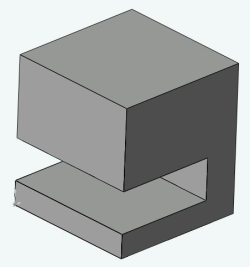
\includegraphics[width=0.7\linewidth]{img/011} \\ \vfill
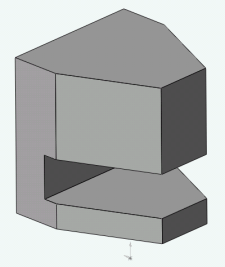
\includegraphics[width=0.7\linewidth]{img/013} \\ \vfill
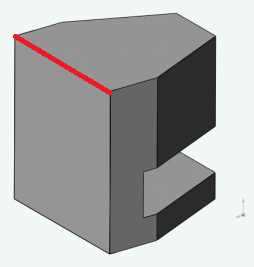
\includegraphics[width=0.7\linewidth]{img/014}
\end{minipage}

\subsection{Création d'un trou}

\begin{minipage}{0.75\linewidth}
\begin{itemize}
 \item Sélectionnez la face supérieure du modèle qui devient verte,
 \item Créer le trou par assistance pour le perçage
 \begin{itemize}
  \item Sélectionnez la fonction volumique,
  \item Choisissez l'onglet données précédentes,
  \item Type de perçage : simple,
  \item Diamètre : 20,
  \item Pour la profondeur, choisir "Condition de fin": "A travers tout",
  \item Cliquez sur suivant puis Terminer.
 \end{itemize}
 \item Nommer la fonction : "trou débouchant".
 \item Positionner le trou,
 \begin{itemize}
  \item Orienter la vue comme ci-contre en choisissant l'icône vue de dessus,
  \item Double cliquer sur la fonction volumique trou débouchant que vous venez de renommer,
  \item Cliquer sur "Éditer l'esquisse",
  \item Créez une ligne de construction passant par les points milieux,
  \item Glissez le centre du cercle sur la ligne de construction puis lâchez,
  \item Cotez la position du trou débouchant.
 \end{itemize}
\end{itemize}
\end{minipage}
\hfill
\begin{minipage}{0.23\linewidth}
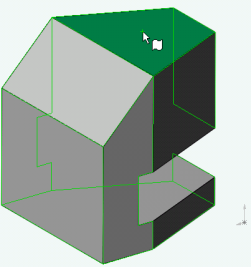
\includegraphics[width=0.7\linewidth]{img/012} \\ \vfill
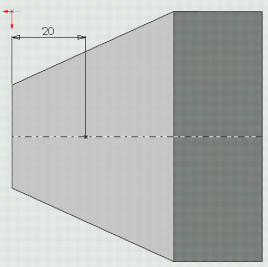
\includegraphics[width=0.7\linewidth]{img/018}
\end{minipage}

\subsection{Création d'un trou lamé}

\textbf{Créer un trou lamé débouchant}

~\

\begin{minipage}{0.75\linewidth}
\begin{itemize}
 \item Sélectionner la surface,
 \item Orientez la vue comme ci-contre,
 \item Sélectionnez la face avant du modèle qui devient verte,
 \item Sélectionnez la fonction volumique,
 \item Choisissez l'onglet données précédentes,
 \item Type de perçage : chambrage (lamage),
 \begin{itemize}
  \item Diamètre perçage: 5,
  \item Ne pas compléter la profondeur,
  \item Diamètre chambrage : 12,
  \item Profondeur : 1,
  \item Cliquez sur suivant puis Terminer,
  \item Condition de fin : Jusqu'à la prochaine surface.
 \end{itemize}
 \item Nommer la fonction volumique : trou lamé
\end{itemize}
\end{minipage}
\hfill
\begin{minipage}{0.23\linewidth}
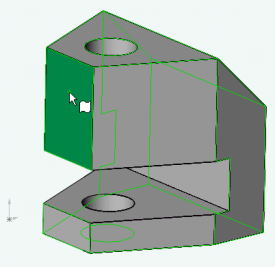
\includegraphics[width=0.9\linewidth]{img/020} \\ \vfill
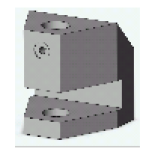
\includegraphics[width=0.9\linewidth]{img/021}
\end{minipage}

\subsection{Création d'un trou lamé}

\textbf{Positionner un trou lamé débouchant}

~\

\begin{minipage}{0.75\linewidth}
\begin{itemize}
 \item Orienter la vue comme ci-contre,
 \item Double cliquer sur la fonction volumique trou lamé,
 \item Cliquer sur "Éditer l'esquisse",
  \begin{itemize}
  \item Créer une ligne de construction passant par l'axe du trou,
  \item Glisser le centre du cercle sur la ligne de construction puis lâchez,
  \item Coter la position du trou lamé : 13 mm.
 \end{itemize}
 \item Sélectionner l'arête
 \begin{itemize}
  \item Orientez la vue comme ci-contre,
  \item Sélectionnez l'arête du trou qui devient verte
 \end{itemize}
 \item Créer le taraudage par «la représentation de filetage »
 \begin{itemize}
  \item Sélectionnez la fonction volumique,
  \item Représentation de filetage,
  \item Entrez la valeur du taraudage : 6,
  \item Indiquez la condition de fin : A travers tout,
  \item Validez : ok
 \end{itemize}
 \item Enregistrer votre travail.
\end{itemize}
\end{minipage}
\hfill
\begin{minipage}{0.23\linewidth}
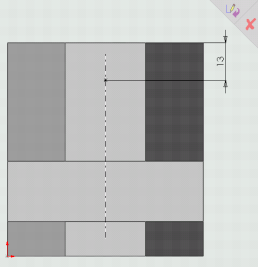
\includegraphics[width=0.9\linewidth]{img/022} \\ \vfill
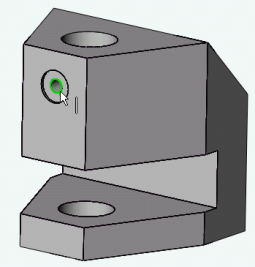
\includegraphics[width=0.9\linewidth]{img/023}
\end{minipage}

\subsection{Modélisation de l'axe}

\begin{minipage}{0.4\linewidth}
A partir de l'esquisse suivante.
\end{minipage}
\hfill
\begin{minipage}{0.58\linewidth}
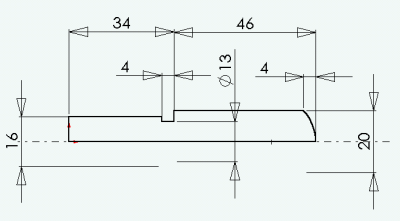
\includegraphics[width=0.9\linewidth]{img/025}
\end{minipage}

\begin{minipage}{0.3\linewidth}
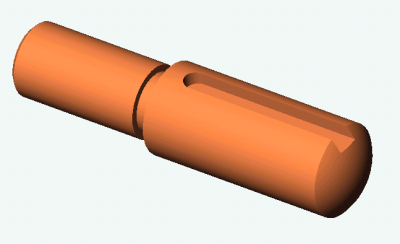
\includegraphics[width=0.9\linewidth]{img/024}
\end{minipage}
\hfill
\begin{minipage}{0.68\linewidth}
Modéliser la pièce suivante. Prendre toutes les décisions nécessaires si les informations permettant la modélisation ne sont pas complètes.
\end{minipage}

\subsection{Modélisation de l'écrou}

\begin{minipage}{0.4\linewidth}
A partir de l'esquisse suivante.
\end{minipage}
\hfill
\begin{minipage}{0.58\linewidth}
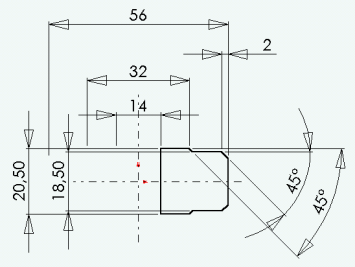
\includegraphics[width=0.8\linewidth]{img/029}
\end{minipage}

\begin{minipage}{0.3\linewidth}
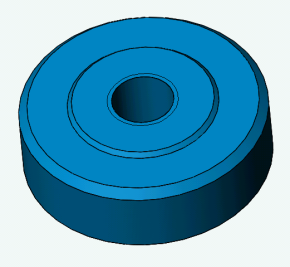
\includegraphics[width=0.7\linewidth]{img/026}
\end{minipage}
\hfill
\begin{minipage}{0.68\linewidth}
Modéliser la pièce suivante. Prendre toutes les décisions nécessaires si les informations permettant la modélisation ne sont pas complètes.
\end{minipage}

\subsection{Modélisation de la vis}

\begin{minipage}{0.4\linewidth}
A partir de l'esquisse suivante.
\end{minipage}
\hfill
\begin{minipage}{0.58\linewidth}
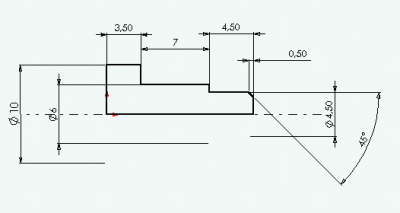
\includegraphics[width=0.9\linewidth]{img/028}
\end{minipage}

\begin{minipage}{0.3\linewidth}
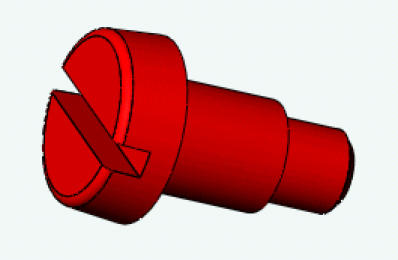
\includegraphics[width=0.8\linewidth]{img/027}
\end{minipage}
\hfill
\begin{minipage}{0.68\linewidth}
Modéliser la pièce suivante. Prendre toutes les décisions nécessaires si les informations permettant la modélisation ne sont pas complètes.
\end{minipage}

\subsection{Mise en mouvement}

A l'aide de l'onglet Meca3D, mettre en place des liaisons sur le système et montrer une mise en mouvement.

\newpage

\section{Cavalier}

Un cavalier est une pièce constituée d'un clou et d'une arche en plastique permettant de guider des câbles.

\begin{minipage}{0.4\linewidth}
 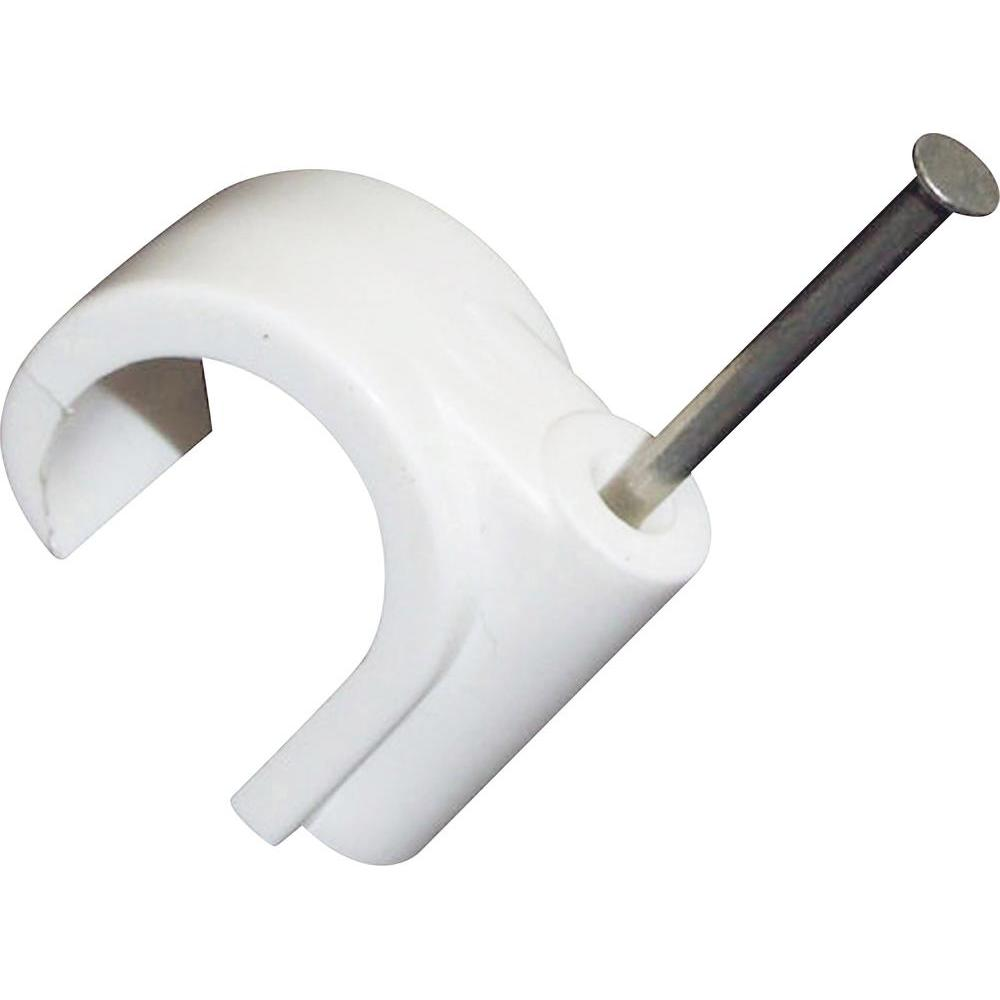
\includegraphics[width=0.9\linewidth]{img/cavalier1}
\end{minipage}\hfill
\begin{minipage}{0.55\linewidth}
 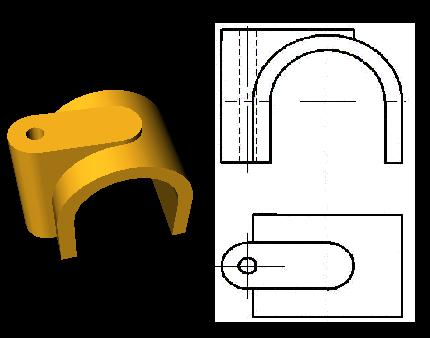
\includegraphics[width=0.9\linewidth]{img/cavalier2}
\end{minipage}

\paragraph{Question 1:} Réaliser l'arbre de construction de l'arche du cavalier.

\end{document}

